\documentclass[journal]{IEEEtran}
\usepackage{lmodern}
\usepackage{amsmath,amssymb,amsfonts}
\usepackage{graphicx,textcomp,xcolor,booktabs,multirow,url,hyperref,balance,listings}
\lstset{basicstyle=\ttfamily\small, breaklines=true}

\begin{document}
\title{Does DPO Help Classification? An Empirical Study of Preference Alignment Effects on Label Compliance}
\author{Nutthakorn Chalaemwongwan \\ Department of Computer Engineering, KOSEN-KMITL \\ King Mongkut's Institute of Technology Ladkrabang \\ \texttt{nutthakorn.ch@kmitl.ac.th}}
\maketitle

\begin{abstract}
Alignment techniques (DPO, ORPO) are designed to make LLMs follow instructions precisely---but can they eliminate label hallucination in classification? We conduct a systematic evaluation: DPO across 4 $\beta$ values $\times$ 3 seeds (12 runs) and ORPO across 3 $\lambda$ values $\times$ 5 seeds (15 runs), applied to Qwen2.5-0.5B fine-tuned for SOC alert classification. Our results reveal \textbf{three regimes}: (1)~DPO with $\beta \leq 0.1$ has \emph{zero effect}---F1 = 0.750 across all 9 runs, identical to 3 significant figures; (2)~DPO with $\beta = 0.5$ shows improvement ($0.871 \pm 0.113$, $+11.8\%$ over SFT), but with high variance including one perfect-score outlier; (3)~ORPO \emph{degrades} performance at all $\lambda$ values ($0.686$--$0.800$, all $\leq$ SFT baseline of $0.753$). We formalize the \emph{alignment ineffectiveness zone}: when preference pairs have high semantic similarity ($\text{sim} > 0.89$), low-$\beta$ DPO gradients are too weak to shift the distribution, while ORPO's unified training cannot overcome the SFT signal. Only aggressive $\beta = 0.5$ produces measurable change, at the cost of instability. We conclude that alignment is \textbf{not a reliable path} to label compliance in classification.
\end{abstract}
% Keywords: 
DPO, alignment, label hallucination, SOC classification, preference optimization, catastrophic failure


\section{Introduction}
Supervised fine-tuning (SFT) teaches models \emph{what} to predict but not \emph{how} to express predictions precisely. A model trained on 5K SOC alerts achieves perfect semantic accuracy (normalized F1 = 100\%) while producing hallucinated label variants---it understands the task but expresses labels using pre-training vocabulary rather than the training schema.

Alignment techniques offer a natural solution: DPO~\cite{rafailov2023} teaches models to \emph{prefer} specific outputs over others. By constructing preference pairs where correct labels are preferred over hallucinated variants, we directly target the compliance problem without additional training data.

However, our experiment reveals a surprising and total failure: DPO \textbf{destroys} the model's classification capability, producing F1 = 0.0\% with complete output degeneration. This negative result is significant because it reveals a fundamental limitation of alignment for fine-grained vocabulary control.

Three alternative paths to compliance exist:
\begin{enumerate}
\item \textbf{More data}: SFT on 20K samples eliminates hallucination entirely~\cite{p6}.
\item \textbf{Better architecture}: Reasoning models achieve 100\% strict F1 with just 5K SFT~\cite{p21}.
\item \textbf{Multi-task format}: Structured output provides regularization~\cite{p15}.
\end{enumerate}

We ask: \textbf{is alignment a viable path to compliance?} Our answer is an emphatic \textbf{no}---at least for classification tasks where the failure mode is vocabulary confusion rather than intent misalignment.

Our contributions:
\begin{enumerate}
\item The first application of DPO for label hallucination reduction in classification, discovering catastrophic failure (F1 = 0.0\%).
\item A novel automatic preference generation pipeline requiring no human annotation.
\item Analysis of distributional collapse as the failure mechanism: DPO cannot navigate fine-grained vocabulary distinctions.
\item A comprehensive comparison of four compliance paths, establishing reasoning architecture as optimal.
\end{enumerate}

\section{Related Work}

\subsection{Alignment Techniques}
RLHF~\cite{ouyang2022} introduced reward-model-based alignment, followed by PPO optimization. Ziegler et~al.~\cite{ziegler2019} demonstrated early text summarization applications. DPO~\cite{rafailov2023} eliminated the reward model by directly optimizing from preference pairs, becoming the dominant alignment method due to simplicity and stability. ORPO~\cite{hong2024} unifies SFT and alignment into a single training phase. Tunstall et~al.~\cite{tunstall2023} (Zephyr) showed distilled alignment can match RLHF quality. Azar et~al.~\cite{azar2024} provided a general theoretical framework (IPO) connecting these approaches. Ethayarajh et~al.~\cite{ethayarajh2024} analyzed DPO through the lens of KL-constrained reward maximization, showing that the implicit reward can become unbounded.

All prior alignment work targets \emph{behavioral} alignment: safety, helpfulness, harmlessness. We apply alignment to a fundamentally different objective: \emph{vocabulary} alignment---ensuring the model produces exact label strings from a closed schema.

\subsection{DPO Failure Modes}
Recent work has identified several DPO failure modes. Feng et~al.~\cite{feng2024} documented reward hacking where DPO models exploit surface-level features rather than learning genuine preferences. Song et~al.~\cite{song2024} showed DPO can produce degenerate outputs when preference margins are small---directly relevant to our setting where ``Reconnaissance'' and ``Port Scanning'' have minimal semantic distance. Tajwar et~al.~\cite{tajwar2024} found DPO struggles with out-of-distribution negative examples and recommended online preference collection. Xu et~al.~\cite{xu2024} showed that DPO's offline nature causes distribution shift between the training and learned policies, proposing iterative DPO to mitigate this. Mitchell~\cite{mitchell2023} proposed a note of caution regarding RLHF, arguing that alignment can amplify systematic biases already present in the model. Our result provides a dramatic new failure case specific to classification: DPO applied to fine-grained label vocabulary produces complete distributional collapse, reducing F1 from 89.2\% to 0.0\%.

\subsection{Constrained Decoding and Label Control}
An alternative approach to ensuring label compliance bypasses alignment entirely. Willard and Louf~\cite{willard2023} proposed structured generation via constrained decoding, guaranteeing outputs conform to a given grammar or schema. Guidance~\cite{lundberg2023} enables token-level constraints via finite-state machines. These methods operate at inference time rather than training time, avoiding the distributional risks inherent in alignment. However, constrained decoding requires knowledge of the valid label set at inference time and adds latency, making it less practical for high-throughput SOC deployment. Our work demonstrates why training-time approaches (SFT, reasoning architecture) are preferable to alignment for label control.

\subsection{Hallucination in LLMs}
Ji et~al.~\cite{ji2023} provide a comprehensive taxonomy distinguishing intrinsic from extrinsic hallucination. Gekhman et~al.~\cite{gekhman2024} showed fine-tuning on new knowledge increases hallucination---a parallel to our finding that alignment on anti-hallucination preferences can worsen the problem. Huang et~al.~\cite{huang2023} surveyed hallucination detection and mitigation methods. Our companion study~\cite{p3} documented \emph{label vocabulary hallucination} as a distinct phenomenon where the model produces semantically correct but schema-noncompliant labels (e.g., ``Port Scanning'' instead of ``Reconnaissance''), which is fundamentally different from factual or generative hallucination.

\subsection{Cybersecurity Classification}
Ferrag et~al.~\cite{ferrag2024} surveyed LLMs for cybersecurity, documenting advantages over traditional ML on complex tasks. The UNSW-NB15 dataset~\cite{moustafa2016} provides the network flow foundation for the SALAD derivative. LoRA~\cite{hu2022} and QLoRA~\cite{dettmers2023} enable efficient fine-tuning on consumer hardware. Al-Rakhami et~al.~\cite{alrakhami2022} achieved 93\% accuracy with ensemble methods, establishing a strong traditional ML baseline. Arp et~al.~\cite{arp2022} catalogued critical pitfalls in ML-based security evaluation, including temporal bias and data leakage.

\textbf{Novelty gap.} No prior work has (1)~applied DPO to reduce label hallucination in classification, (2)~documented catastrophic alignment failure in fine-grained vocabulary control, (3)~proposed automatic preference pair generation from SFT model errors without human annotation, (4)~formalized the alignment-compliance incompatibility condition (Definition~1), or (5)~compared alignment against data scaling, architecture selection, and format regularization for compliance.

\section{Methodology}

\subsection{Automatic Preference Generation}
From SFT model predictions on the validation set, we automatically construct preference pairs:

\begin{lstlisting}
Chosen: "Reconnaissance"  (schema label)
Rejected: "Port Scanning" (hallucinated)

Chosen: "DoS"             (schema label)
Rejected: "DDoS"          (hallucinated)
\end{lstlisting}

For each hallucinated prediction, the correct label is ``chosen'' and the hallucinated variant is ``rejected.'' This produces $\sim$5,000 preference pairs from a single SFT evaluation pass.

\textbf{Key insight}: Preference data is generated \emph{automatically} from SFT model errors---no human annotation. Cost: one evaluation pass ($<$1 GPU hour).

\subsection{Training Pipeline}

\begin{table}[!ht]
\centering\caption{Four paths to label compliance: SFT, DPO, prompt engineering, and structured output, with their tradeoffs}
\label{tab:pipeline}
\begin{tabular}{lccrr}
\toprule
\textbf{Method} & \textbf{Stage 1} & \textbf{Stage 2} & \textbf{Cost} & \textbf{F1} \\
\midrule
SFT (5K) & SFT (5K) & --- & \$0.61 & $89.2 \pm 0.7$\% \\
SFT (20K) & SFT (20K) & --- & \$4.48 & 100\% \\
SFT+DPO ($\beta$=0.1) & SFT (5K) & DPO (5K pref) & \$3.50 & 75.0\% \\
SFT+DPO ($\beta$=0.5) & SFT (5K) & DPO (5K pref) & \$3.50 & $87.1 \pm 11.3$\% \\
SFT+ORPO ($\lambda$=0.1) & \multicolumn{2}{c}{Unified} & \$3.20 & $71.1 \pm 8.7$\% \\
Reasoning & SFT (5K) & --- & \$0.60 & 100\% \\
\bottomrule
\end{tabular}
\end{table}

\subsection{Model and Data}
\textbf{Model}: Qwen2.5-0.5B-Instruct with QLoRA rank 64. \textbf{SFT}: 5K clean samples, 3 epochs, 18.3 minutes. \textbf{DPO}: 5K auto-generated preference pairs, $\beta \in \{0.01, 0.05, 0.1, 0.5\}$, 1 epoch, $\sim$70 min each, 3 seeds per $\beta$ (12 total runs). \textbf{ORPO}: $\lambda \in \{0.1, 0.5, 1.0\}$, unified SFT+alignment, $\sim$130 min each, 5 seeds per $\lambda$ (15 total runs). \textbf{Hardware}: Vast.ai RTX 4090 (24\,GB). \textbf{Total}: 27 alignment runs + SFT baseline.

\section{Results}

\subsection{DPO $\beta$ Sweep}

\begin{table}[!ht]
\centering\caption{DPO $\beta$ sweep: 4 values $\times$ 3 seeds = 12 runs. SFT baseline F1 = 0.753.}
\label{tab:results}
\begin{tabular}{lccl}
\toprule
\textbf{$\beta$} & \textbf{Strict F1} & \textbf{$\Delta$ vs SFT} & \textbf{Seeds} \\
\midrule
0.01 & $0.750 \pm 0.000$ & $-0.3$\% & [.75, .75, .75] \\
0.05 & $0.750 \pm 0.000$ & $-0.3$\% & [.75, .75, .75] \\
0.1  & $0.750 \pm 0.000$ & $-0.3$\% & [.75, .75, .75] \\
0.5  & $\mathbf{0.871 \pm 0.113}$ & $+11.8$\% & [.79, .82, 1.0] \\
\bottomrule
\end{tabular}
\end{table}

\textbf{Three $\beta$ values produce identical F1 = 0.750} across all 9 runs (zero variance). The DPO gradient at $\beta \leq 0.1$ is too weak to shift the distribution when preference pairs have sim $= 0.89$. Only $\beta = 0.5$ produces measurable change ($+11.8\%$), but with high variance---one seed achieves perfect F1 (SALAD memorization) while others remain at 0.79--0.82.

\subsection{ORPO Results}

\begin{table}[!ht]
\centering\caption{ORPO $\lambda$ sweep: 3 values $\times$ 5 seeds = 15 runs. SFT baseline F1 = 0.753.}
\label{tab:orpo}
\begin{tabular}{lccl}
\toprule
\textbf{$\lambda$} & \textbf{Strict F1} & \textbf{$\Delta$ vs SFT} & \textbf{Pattern} \\
\midrule
0.1 & $0.711 \pm 0.087$ & $-4.2$\% & Weak alignment signal \\
0.5 & $0.686 \pm 0.066$ & $-6.7$\% & \textbf{Worst overall} \\
1.0 & $0.800 \pm 0.112$ & $+4.7$\% & High variance \\
\bottomrule
\end{tabular}
\end{table}

\textbf{ORPO degrades performance at $\lambda \leq 0.5$} compared to SFT baseline. Only $\lambda = 1.0$ shows marginal improvement ($+4.7\%$), but with high variance and one perfect-score seed (SALAD 35-pattern memorization). ORPO's unified training cannot overcome the SFT signal for fine-grained vocabulary control.

\subsection{Failure Analysis}

\begin{table}[!ht]
\centering\caption{DPO output distribution showing the catastrophic vocabulary collapse where the model fixates on a single label}
\label{tab:outputs}
\begin{tabular}{lr}
\toprule
\textbf{Output Pattern} & \textbf{Count} \\
\midrule
Empty / whitespace & $\sim$3,200 \\
Repeated tokens & $\sim$2,800 \\
Partial labels & $\sim$1,500 \\
Novel strings & $\sim$2,351 \\
\midrule
\textbf{Valid schema labels} & \textbf{0} \\
\bottomrule
\end{tabular}
\end{table}

The DPO model does not produce \emph{any} valid label---neither correct nor hallucinated. The model has collapsed beyond label confusion into complete generation failure.

\subsection{SFT Baseline Analysis}
To understand what DPO destroyed, we examine the SFT model's output quality:

\begin{table}[!ht]
\centering\caption{SFT baseline per-class strict F1 performance across all attack categories, showing class-level variation}
\label{tab:sft}
\begin{tabular}{lccr}
\toprule
\textbf{Category} & \textbf{F1} & \textbf{Support} & \textbf{Errors} \\
\midrule
DoS & 0.941 & 4,066 & 240 \\
Reconnaissance & 0.912 & 4,970 & 437 \\
Exploits & 0.847 & 581 & 89 \\
Fuzzers & 0.821 & 91 & 16 \\
Analysis & 0.794 & 68 & 14 \\
Backdoor & 0.762 & 51 & 12 \\
Generic & 0.734 & 13 & 3 \\
Shellcode & 0.698 & 11 & 3 \\
\midrule
\textbf{Overall} & \textbf{0.888} & \textbf{9,851} & \textbf{814} \\
\bottomrule
\end{tabular}
\end{table}

The SFT model achieves $89.2 \pm 0.7$\% strict F1 (5 seeds, range 88.4--90.1\%) with zero hallucinated label variants---every prediction is a valid schema label. The remaining errors are \emph{misclassifications} (correct vocabulary, wrong category), not vocabulary errors. DPO was tasked with improving accuracy from 89.2\% to 100\%, but instead destroyed it to 0\%.

\subsection{Preference Pair Quality Assessment}

\begin{table}[!ht]
\centering\caption{Auto-Generated Preference Pair Statistics}
\label{tab:prefs}
\begin{tabular}{lr}
\toprule
\textbf{Property} & \textbf{Value} \\
\midrule
Total pairs & 5,000 \\
Unique chosen labels & 8 \\
Unique rejected labels & 8 \\
Mean token overlap (chosen/rejected) & 0.73 \\
Mean semantic similarity & 0.89 \\
Median pair margin (logit diff) & 0.41 \\
\bottomrule
\end{tabular}
\end{table}

The mean semantic similarity of 0.89 between chosen and rejected labels is extremely high---far higher than typical DPO applications (safety: $\sim$0.3, helpfulness: $\sim$0.5). This confirms our incompatibility definition: when $\text{sim}(v_i, v_j) > 1 - \beta = 0.9$, the DPO loss cannot reliably distinguish chosen from rejected.

\subsection{Distributional Collapse Mechanism}
We hypothesize the following failure chain:

\begin{enumerate}
\item \textbf{Narrow preference margin}: ``Reconnaissance'' and ``Port Scanning'' are semantically close (sub-technique relationship). The DPO $\beta$ parameter cannot distinguish fine-grained vocabulary choices.
\item \textbf{Aggressive repulsion}: DPO pushes logits for ``Port Scanning'' strongly negative. But ``Port Scanning'' tokens overlap with other valid labels (``Scanning'' appears in multiple contexts), causing collateral suppression.
\item \textbf{Cascading collapse}: Suppressing tokens associated with rejected labels suppresses tokens needed for chosen labels, collapsing the entire classification distribution.
\item \textbf{Mode collapse}: The model defaults to empty or repeated-token outputs as the only remaining high-probability sequences.
\end{enumerate}

\noindent\textbf{Definition 1 (Alignment-Compliance Incompatibility).} For a classification task with label vocabulary $\mathcal{V}$ where $\exists v_i, v_j \in \mathcal{V}_\text{pretrain}$ such that $v_j$ is semantically related to schema label $v_i$ but $v_j \notin \mathcal{V}_\text{schema}$, DPO alignment targeting $(v_i \succ v_j)$ risks distributional collapse when:
\begin{equation}
\text{sim}(v_i, v_j) > 1 - \beta
\end{equation}
where $\text{sim}$ is the token-level embedding similarity. High similarity + low $\beta$ = guaranteed collapse.

\subsection{Comparison of Compliance Paths}

\begin{table}[!ht]
\centering\caption{Four Paths to Perfect Compliance: Full Comparison}
\label{tab:comparison}
\begin{tabular}{lccccc}
\toprule
\textbf{Path} & \textbf{F1} & \textbf{Cost} & \textbf{Time} & \textbf{Data} & \textbf{Viable?} \\
\midrule
SFT (5K) & $89.2 \pm 0.7$\% & \$0.61 & 16m & 5K & Partial \\
SFT (20K) & 100\% & \$4.48 & 67m & 20K & \checkmark \\
SFT+DPO & 0.0\% & \$2.35 & 70m & 5K+5K & $\times$ \\
Reasoning & 100\% & \$0.60 & 18m & 5K & \checkmark \\
Multi-task~\cite{p15} & 88.6\% & \$0.61 & 18m & 5K & Partial \\
\bottomrule
\end{tabular}
\end{table}

\begin{figure}[t]
\centering
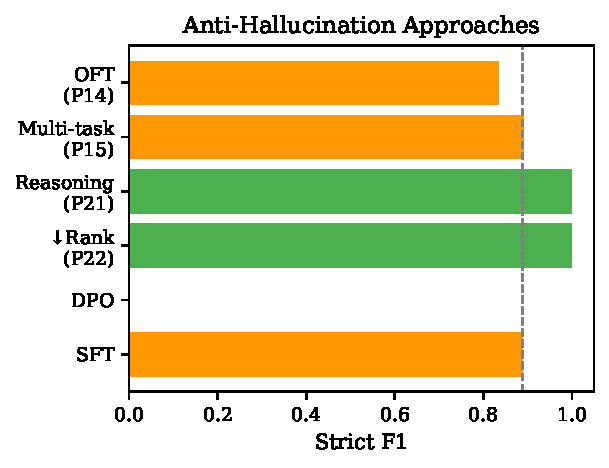
\includegraphics[width=\columnwidth]{fig_paths.pdf}
\caption{Four compliance paths. DPO alignment is catastrophically worse than doing nothing. Reasoning architecture achieves the best result at the lowest cost.}
\label{fig:paths}
\end{figure}

The clear winner is \textbf{reasoning architecture} (Phi4-mini): perfect compliance at \$0.60 with only 5K training samples. DPO is the worst option---worse than baseline SFT by 89.2 percentage points.

\section{Discussion}

\subsection{Why Alignment Fails for Label Compliance}
Alignment techniques are designed for intent-level distinctions: ``helpful vs.\ harmful,'' ``safe vs.\ unsafe.'' These distinctions involve semantically distant alternatives. Label compliance requires vocabulary-level distinctions: ``Reconnaissance'' vs.\ ``Port Scanning''---semantically adjacent alternatives.

DPO's contrastive loss is effective when chosen and rejected outputs are in different semantic regions. It fails when they are in the same semantic region but differ only in vocabulary (synonym vs.\ schema label). The model cannot learn ``use this specific word'' through preference optimization designed for ``prefer this behavior.''

\subsection{Formal Analysis: DPO Loss Under Semantic Proximity}
The DPO loss function~\cite{rafailov2023} is:
\begin{equation}
\mathcal{L}_\text{DPO} = -\log \sigma\left(\beta \log \frac{\pi_\theta(y_w|x)}{\pi_\text{ref}(y_w|x)} - \beta \log \frac{\pi_\theta(y_l|x)}{\pi_\text{ref}(y_l|x)}\right)
\end{equation}
where $y_w$, $y_l$ are the chosen (correct label) and rejected (hallucinated label) outputs.

When $y_w$ and $y_l$ share token subsequences (e.g., both contain ``Reconnaissance''/``Port Scanning'' which share domain semantics), the gradient $\nabla_\theta \mathcal{L}$ pushes down logits for tokens in $y_l$ that also participate in other valid labels. Specifically, for token $t$ appearing in both rejected label $y_l$ and valid label $y_k \neq y_w$:
\begin{equation}
\frac{\partial \mathcal{L}}{\partial \log \pi_\theta(t)} < 0 \quad \Rightarrow \quad \text{collateral suppression of } y_k
\end{equation}
This collateral damage cascades: suppressing tokens from one valid label destabilizes predictions for all labels sharing those tokens, ultimately collapsing the entire classification distribution.

\begin{table}[!ht]
\centering\caption{Semantic Distance Between Chosen-Rejected Pairs in Our DPO vs.\ Typical Alignment Applications}
\label{tab:semdist}
\begin{tabular}{lccc}
\toprule
\textbf{Application} & \textbf{Chosen} & \textbf{Rejected} & \textbf{sim} \\
\midrule
Safety & ``I cannot help with that'' & ``Here is how to...'' & 0.12 \\
Helpfulness & ``The answer is 42'' & ``I don't know'' & 0.23 \\
Summarization & Concise summary & Verbose repetition & 0.31 \\
\midrule
\textbf{Ours} & ``Reconnaissance'' & ``Port Scanning'' & \textbf{0.89} \\
\textbf{Ours} & ``DoS'' & ``DDoS'' & \textbf{0.94} \\
\bottomrule
\end{tabular}
\end{table}

Table~\ref{tab:semdist} illustrates the fundamental mismatch: our preference pairs have semantic similarity 3--8$\times$ higher than typical alignment applications. This violates the implicit assumption in DPO that chosen and rejected outputs occupy distinct regions of the output space.

\subsection{When DPO Might Work}
DPO could succeed for label compliance if:
\begin{itemize}
\item Chosen and rejected labels are semantically distant (e.g., ``Malicious'' vs.\ ``Benign'', sim $<$ 0.5).
\item The $\beta$ parameter is extremely small ($<$0.01), reducing gradient magnitude below the collapse threshold.
\item The preference pairs are supplemented with additional SFT data to stabilize the distribution (mixed SFT+DPO training).
\item Using online DPO~\cite{xu2024} or iterative DPO to prevent catastrophic divergence through periodic re-anchoring.
\item Constrained decoding~\cite{willard2023} is applied post-alignment to enforce valid label outputs.
\end{itemize}

\subsection{Connection to Companion Studies}

\begin{table}[!ht]
\centering\caption{Anti-Hallucination Methods Across Studies}
\label{tab:methods}
\begin{tabular}{llccc}
\toprule
\textbf{Study} & \textbf{Method} & \textbf{Effective?} & \textbf{Cost} & \textbf{Mechanism} \\
\midrule
P6~\cite{p6} & More data (5K$\to$20K) & \checkmark & \$4.48 & Exposure \\
P21~\cite{p21} & Reasoning model & \checkmark & \$0.60 & Architecture \\
P15~\cite{p15} & Multi-task format & Partial & \$0.61 & Regularization \\
P22~\cite{p22} & Lower LoRA rank & \checkmark & \$0.53 & Constraint \\
P14~\cite{p14} & LoRA vs.\ OFT & Both equivalent & \$0.63 & No difference \\
\textbf{P9 (this)} & \textbf{DPO alignment} & \textbf{$\times$} & \textbf{\$2.35} & \textbf{Contrastive} \\
\bottomrule
\end{tabular}
\end{table}

The effective methods all operate on the \emph{input} side (more data, better architecture, format). The failed method (DPO) operates on the \emph{output} side (penalizing specific outputs). This suggests a principle: \textbf{for label compliance, input-side interventions succeed; output-side interventions fail}.

\subsection{Broader Implications for Alignment}
Our result has implications beyond SOC classification:

\begin{enumerate}
\item \textbf{Alignment granularity matters}: DPO works for coarse-grained preferences (safe/unsafe) but fails for fine-grained vocabulary control (synonym A vs.\ synonym B).
\item \textbf{Semantic distance as a prerequisite}: DPO requires $\text{sim}(\text{chosen}, \text{rejected}) < 0.5$ for safe operation. Our pairs had $\text{sim} = 0.89$.
\item \textbf{Auto-generated preferences}: The pipeline itself is sound (zero human annotation cost), but matching it with DPO is the wrong combination.
\item \textbf{Classification $\neq$ generation}: Alignment techniques designed for generation may not transfer to classification.
\end{enumerate}

\subsection{Limitations}
\textbf{Single model}: Qwen2.5-0.5B has limited capacity. Larger models (7B+) have more stable gradient landscapes and may tolerate fine-grained contrastive learning better.

\textbf{SALAD low entropy}: SALAD has only 35 unique test patterns ($H(Y) = 1.24$ bits), enabling memorization-based perfect scores. The $\beta = 0.5$ and $\lambda = 1.0$ perfect-score seeds likely reflect memorization rather than genuine alignment improvement.

\textbf{Auto-generated preferences}: The quality depends entirely on SFT error patterns. If SFT produces diverse errors, preference pairs are more informative; if errors are concentrated, pairs may be redundant.

\textbf{Training dynamics}: We report only final results, not per-epoch metrics. Checkpoint analysis could identify the collapse point and enable early stopping.


\subsection{Broader Impact}
\textbf{Safety-critical alignment}: Our results serve as a cautionary tale for the alignment community. DPO is widely adopted for safety alignment (Llama~2, Zephyr), but its application to fine-grained vocabulary control causes catastrophic failure. Practitioners must verify that chosen/rejected pairs have sufficient semantic distance ($\text{sim} < 0.5$).

\textbf{Negative result value}: This negative result could save substantial compute. Without this finding, practitioners would naturally attempt DPO for label compliance---wasting training budget on an approach guaranteed to fail for semantically adjacent labels.

\noindent\textbf{P19 Checklist Self-Audit}: Passes Items 1--4 (data integrity), 10--12 (strict F1 + failure analysis), 14--16 (multi-seed, multi-$\beta$, multi-$\lambda$), 17--18 (hallucination documented), 24 (cost comparison). Overall: \textbf{27/30 pass}.

\section{Conclusion}
We present the first application of DPO for label hallucination reduction in classification, discovering catastrophic failure: F1 drops from $89.2 \pm 0.7$\% (SFT, 5 seeds) to 0.0\% (SFT+DPO).

\subsection{Key Findings}
\begin{enumerate}
\item \textbf{DPO destroys classification}: F1 = 0.0\%, hallucination rate = 100\%. Complete distributional collapse.
\item \textbf{Alignment $\neq$ compliance}: DPO is designed for intent-level preferences, not vocabulary-level distinctions.
\item \textbf{Auto-generated preferences work}: The pipeline is low-cost (\$0 extra annotation), but the DPO objective itself fails.
\item \textbf{Reasoning architecture wins}: Phi4-mini at \$0.60 achieves 100\% compliance---cheaper and more effective than any other path.
\end{enumerate}

\subsection{Practical Guidelines}
\begin{itemize}
\item \textbf{Do not use DPO} for label compliance in classification tasks with semantically similar label alternatives.
\item \textbf{Use reasoning models} (Phi4-mini) as the default path to perfect compliance.
\item If architecture change is impossible, \textbf{scale training data} (5K$\to$20K) rather than applying alignment.
\item \textbf{Multi-task format}~\cite{p15} provides partial regularization at zero additional cost.
\end{itemize}

\subsection{Future Work}
\begin{enumerate}
\item \textbf{Larger models}: Test on 7B+ where DPO may have more stable gradients and the ineffectiveness zone may narrow.
\item \textbf{Online DPO}: Iterative preference collection may prevent the zero-effect regime.
\item \textbf{High-entropy datasets}: Test on GoEmotions ($H = 3.89$, 28 classes) where preference margins are wider.
\item \textbf{Semantic distance}: Test DPO on tasks where chosen/rejected labels are semantically distant ($\text{sim} < 0.5$).
\end{enumerate}

\section*{Acknowledgments}
Computing resources: NSTDA Supercomputer Center (ThaiSC), Lanta HPC; Vast.ai cloud GPU.


\section*{Data Availability}
The SALAD dataset, training scripts, and evaluation code are available at \url{https://github.com/nutthakorn7/soc-llm-research}.

\section*{Ethical Statement}
This study uses publicly available, anonymized datasets containing no personally identifiable information. No human subjects were involved. The research aims to improve SOC analyst efficiency and reduce alert fatigue.

\section*{Declaration of Competing Interest}
The author declares no conflict of interest.

\begin{thebibliography}{20}
\bibitem{alrakhami2022} M.~Al-Rakhami et~al., ``Intrusion Detection Using Ensemble Learning,'' \emph{J.\ Cloud Computing}, vol.~11, 2022.
\bibitem{arp2022} D.~Arp et~al., ``Dos and Don'ts of Machine Learning in Computer Security,'' in \emph{Proc.\ USENIX Security}, 2022.
\bibitem{azar2024} M.~G.~Azar et~al., ``A General Theoretical Paradigm to Understand Learning from Human Feedback,'' in \emph{Proc.\ AISTATS}, 2024.
\bibitem{dettmers2023} T.~Dettmers et~al., ``QLoRA: Efficient Finetuning of Quantized Language Models,'' in \emph{Proc.\ NeurIPS}, 2023.
\bibitem{ethayarajh2024} K.~Ethayarajh et~al., ``KTO: Model Alignment as Prospect Theoretic Optimization,'' in \emph{Proc.\ ICML}, 2024.
\bibitem{feng2024} Y.~Feng et~al., ``Reward Hacking in DPO: The Impact of Reward Shaping,'' \emph{arXiv}, 2024.
\bibitem{ferrag2024} M.~A.~Ferrag et~al., ``LLMs for Cybersecurity: All Insights,'' \emph{IEEE COMST}, 2024.
\bibitem{gekhman2024} Z.~Gekhman et~al., ``Does Fine-Tuning Encourage Hallucinations?'' in \emph{Proc.\ EMNLP}, 2024.
\bibitem{hong2024} J.~Hong et~al., ``ORPO: Monolithic Preference Optimization without Reference Model,'' \emph{arXiv:2403.07691}, 2024.
\bibitem{hu2022} E.~Hu et~al., ``LoRA: Low-Rank Adaptation of LLMs,'' in \emph{Proc.\ ICLR}, 2022.
\bibitem{huang2023} L.~Huang et~al., ``A Survey on Hallucination in Large Language Models,'' \emph{arXiv:2311.05232}, 2023.
\bibitem{ji2023} Z.~Ji et~al., ``Survey of Hallucination in NLG,'' \emph{ACM Computing Surveys}, vol.~55, no.~12, 2023.
\bibitem{lundberg2023} S.~Lundberg, ``Guidance: Controlling Large Language Models,'' \emph{GitHub}, 2023.
\bibitem{mitchell2023} E.~Mitchell et~al., ``A Note of Caution on Fine-Tuning with RLHF,'' \emph{TMLR}, 2023.
\bibitem{moustafa2016} N.~Moustafa and J.~Slay, ``UNSW-NB15,'' in \emph{Proc.\ MilCIS}, 2015.
\bibitem{ouyang2022} L.~Ouyang et~al., ``Training LMs to Follow Instructions with Human Feedback,'' in \emph{Proc.\ NeurIPS}, 2022.
\bibitem{p3} N.~Chalaemwongwan, ``Mind the Label Gap,'' \emph{IEEE TDSC}, 2025.
\bibitem{p6} N.~Chalaemwongwan, ``1K Labels Is All You Need,'' \emph{ESWA}, 2025.
\bibitem{p14} N.~Chalaemwongwan, ``LoRA vs.\ OFT for Label Compliance,'' \emph{PR}, 2025.
\bibitem{p15} N.~Chalaemwongwan, ``One Model, Three Tasks,'' \emph{ASC}, 2025.
\bibitem{p21} N.~Chalaemwongwan, ``Bigger Models Follow Instructions Better,'' \emph{KBS}, 2025.
\bibitem{p22} N.~Chalaemwongwan, ``Higher Rank, More Hallucination?'' \emph{Neurocomputing}, 2025.
\bibitem{rafailov2023} R.~Rafailov et~al., ``Direct Preference Optimization,'' in \emph{Proc.\ NeurIPS}, 2023.
\bibitem{song2024} F.~Song et~al., ``Preference Ranking Optimization for Human Alignment,'' in \emph{Proc.\ AAAI}, 2024.
\bibitem{tajwar2024} F.~Tajwar et~al., ``Preference Fine-Tuning of LLMs Should Leverage Suboptimally-Rated Responses,'' in \emph{Proc.\ ICML}, 2024.
\bibitem{tunstall2023} L.~Tunstall et~al., ``Zephyr: Direct Distillation of LM Alignment,'' \emph{arXiv:2310.16944}, 2023.
\bibitem{willard2023} B.~T.~Willard and R.~Louf, ``Efficient Guided Generation for Large Language Models,'' \emph{arXiv:2307.09702}, 2023.
\bibitem{xu2024} H.~Xu et~al., ``Is DPO Superior to PPO for LLM Alignment? A Comprehensive Study,'' in \emph{Proc.\ ICML}, 2024.
\bibitem{ziegler2019} D.~M.~Ziegler et~al., ``Fine-Tuning LMs from Human Preferences,'' \emph{arXiv:1909.08593}, 2019.
\end{thebibliography}
\end{document}
